\documentclass[utf8, a4paper, 11pt, parskip, pointlessnumbers]{scrreprt}

%%%%%%%%%%%%%%%%%%%%%%Kompilieren dieser Latex Vorlage%%%%%%%%%%%%%%%%%%%%%%%
%How to configure Texmaker's Quick Build: 
%1. Options -> configure Texmaker
%2. Commands Tab on side -> PDF viewer -> tick internal viewer and integrate in Texmaker
%3. Quick-Build Tab on side -> user defined
%4. Copy this: pdflatex -synctex=1 -interaction=nonstopmode %.tex|makeindex %.nlo -s nomencl.ist -o %.nls|pdflatex -synctex=1 -interaction=nonstopmode %.tex|bibtex %|"C:/Program Files (x86)/Adobe/Reader 11.0/Reader/AcroRd32.exe" %.pdf
%5.Ccheck that the file path to ADOBE reader is correct for your computer

%%%%%%%%%%%%%%%%%%%%%%%%%%%%%%%%%%%Präambel%%%%%%%%%%%%%%%%%%%%%%%%%%%%%%%%%%%%
%%%%%%%%%%%%%%%%%%%%%%%%%%%%%%%%%%%Präambel%%%%%%%%%%%%%%%%%%%%%%%%%%%%%%%%%%%%

%%%%%%%%%%%%%%%%%%%%% 
%      Pakete       %
%%%%%%%%%%%%%%%%%%%%%
\usepackage[utf8]{inputenc} % Textcodierung UTF-8
\usepackage[english]{babel} % Deutsche Lokalisierung
\usepackage[T1]{fontenc} % Zeichensatzkodierung
\usepackage[scaled]{helvet} % Helvetica Schriftart
\usepackage{nicefrac} % Darstellung von Brüchen in Formeln
\usepackage{alphalph} % Option mit Buchstaben anstatt mit Zahlen zu zählen (z.B. für Seitenzahlen)
\usepackage{array}
\usepackage{amssymb}
\usepackage{amsmath} % Darstellung von Formeln
\usepackage{amsthm} % Darstellung von Mathematischen Theoremen
\usepackage{threeparttable} % Einbindung von Tabellen mit Fußnoten
\usepackage{caption} % Customise Bildunter- und Tabellenüberschriften
\usepackage{tocloft} % Formatierung von Inhaltsverzeichnis, Abbildungs- und Tabellenverzeichnis
\usepackage{booktabs} % Customise Tabellen mit Extra-Kommandos
\usepackage{enumitem} % Formatierung von Listen (itemize, enumerate and description)
\usepackage{geometry} % Einstellung der Seitengeometrie
\usepackage{siunitx} % SI-Einheiten Paket
\usepackage{color} % Für Matlab Code
\usepackage{colortbl} % Benutzung von Farben in Tabellen
\usepackage{setspace} % Zeilenabstand
\usepackage{multirow} % Tabellen Paket
\usepackage{chngcntr} % Nummerierungen
\usepackage{natbib} % Bibliographie Paket
\usepackage{graphicx} % Zur Einbindung von Abbildungen
\usepackage{epstopdf} % Möglichkeit auch .eps Dateien einzubinden
\usepackage[hyphens]{url} % URL-Paket mit Option zur Zeilentrennung nach Gedanken-/Bindestrichen
\usepackage{hyperref} % Zur Erzeugung von hyperlinks im Dokument
\usepackage[raggedleft]{titlesec} % Formatierung von Kapitel-Überschriften
\usepackage[toc,page]{appendix} % Customise den Anhang
\usepackage{listings} % Einbinden von Listen
\usepackage{nomencl} % Nomenklatur 
\usepackage{ifthen} % Für Bedingungen
\usepackage{fancyhdr} % Header & Footer Package
\usepackage[boxed,chapter]{algorithm} % Einbindung von Algorithmen als Pseudo-Code (schwarze Box um den Pseudo-Code und Nummerierung mit Einbeziehung der Kapitel Nummer
\usepackage{algpseudocode}% http://ctan.org/pkg/algorithmicx
\usepackage{tabto} % Tabulatoren
\usepackage{parskip} % Kontrolle der Absatzgröße
\usepackage[absolute]{textpos} % Positionierung

%%%%%%%%%%%%%%%%%%%%% 
%   Einstellungen   %
%%%%%%%%%%%%%%%%%%%%%
\geometry{a4paper, top=30mm, bottom=35mm, inner=35mm, outer=25mm, headsep=11mm, footskip=21mm} % Seitenformatierung

\renewcommand*\familydefault{\sfdefault} % Schriftart-Einstellung: Sans serif
\DeclareOldFontCommand{\bf}{\normalfont\bfseries}{\mathbf} % define command \bf  (used by bibliography I think)
\linespread{1.5}\selectfont % Zeilenabstand
\sloppy % Silbentrennungeinstellung: möglichst selten trennen

%Einstellungen für Seitenumbrüche  
\interfootnotelinepenalty=9999 % Kein Seitenumbruch innerhalb einer Fußnote!
\clubpenalty0
\widowpenalty0
\displaywidowpenalty0

% Kapitel und Unterkapitel Formatierung
\titleformat{\chapter}{\Large\bfseries}{\Large\bfseries\thechapter}{6pt}{\Large}
\titleformat{\section}{\large\bfseries}{\large\bfseries\thesection}{6pt}{\large}
\titleformat{\subsection}{\normalsize\bfseries}{\normalsize\bfseries\thesubsection}{6pt}{\normalsize}
\titlespacing*{\chapter}{0pt}{-35pt}{0pt} % Vertikale Abstände
\titlespacing*{name=\chapter,numberless}{0pt}{-35pt}{0pt}
\titlespacing*{\section}{0pt}{0pt}{0pt}
\titlespacing*{\subsection}{0pt}{0pt}{0pt}

% Abbildungs-/Tabelleneinstellungen
\captionsetup{labelfont={bf}} % Abbildung/Tabelle fett drucken

% SI-Einheit Einstellungen
\sisetup{per-mode = symbol}%
\sisetup{detect-weight = true}

% Definition von Befehlen, um Unterkapitel des Anhangs nicht ins Inhaltsverzeichnis aufzunehmen
\newcommand{\stoptocwriting}{\addtocontents{toc}{\protect\setcounter{tocdepth}{-5}}} % Stopt die Aufnahme von Kapitelnamen ins Inhaltsverzeichnis
\newcommand{\resumetocwriting}{\addtocontents{toc}{\protect\setcounter{tocdepth}{\arabic{tocdepth}}}} % Nimmt die Aufnahme von Kapitelnamen ins Inhaltsverzeichnis wieder auf
  
% Einbindung von Matlab-Code mit den Matlab-Farben
\definecolor{mlgreen}{rgb}{.035,.6,.251}
\definecolor{mlviolett}{rgb}{.643,.259,.804}
\lstdefinestyle{mlab}{language=Matlab, 
otherkeywords={},
deletekeywords={def,real,length,gamma,zeros,figure,subplot,plot,xlabel,ylabel,zlabel,sin,pi,diff,size,meshgrid,legend,surf,min,trapz,cos,eig,exp,abc},
numbers=left,
numberstyle=\tiny,%5
basicstyle={\ttfamily},%
keywordstyle={\color{blue}},%
commentstyle=\color{mlgreen},%
stringstyle=\color{mlviolett},%
breaklines=true,%
showstringspaces=false,%
numberbychapter=true, %
xleftmargin=15pt
 }

% Einstellungen für das Symbolverzeichnis
\newlength{\nomgroupstartsep}
\setlength{\nomgroupstartsep}{16pt}

\newlength{\nomintermsep}
\setlength{\nomintermsep}{-\parsep}


\renewcommand{\nomgroup}[1]{%
	\ifthenelse{\equal{#1}{A}}{\item[\textbf{Abbreviations}]}{%
	\ifthenelse{\equal{#1}{I}}{\vspace{16pt} \item[\textbf{Indices}]}{%
	\ifthenelse{\equal{#1}{G}}{\vspace{16pt} \item[\textbf{Greek Symbols}]}{%
	\ifthenelse{\equal{#1}{L}}{\vspace{16pt} \item[\textbf{Latin Symbols}]}}}}

}
\setlength{\nomlabelwidth}{.2\hsize} % Abstand zwischen Variable und Erklärung
\setlength{\nomitemsep}{-\parsep} % Zeilenabstand verkleinern
\renewcommand{\nomlabel}[1]{#1 \dotfill} % Punkte zw. Abkürzung und Erklärung
\newcommand{\nomunit}[1]{\renewcommand{\nomentryend}{\dotfill #1}}
\makenomenclature % Erstellen des Symbolverzeichnisses

% Einstellung Hyperlink
\hypersetup{colorlinks,citecolor=black,filecolor=black,linkcolor=black,urlcolor=black} % Hyperlink Einstellungen

% Einstellung Algorithmus Package
\floatname{algorithm}{Algorithmus} % Unterschrift eines Algorithmus ist auf Deutsch

% Header & Footer Einstellungen
  \pagestyle{fancy} %eigener Seitenstil
\renewcommand{\chaptermark}[1]{\markboth{\thechapter~ #1}{}}
\renewcommand{\sectionmark}[1]{\markright{\thechapter~ #1}}

  \fancyhf{}%alle Kopf- und Fußzeilenfelder bereinigen
  \renewcommand{\headrulewidth}{0.4pt}%obere Trennlinie
  \fancyhead[R]{\small{\nouppercase\leftmark}}
  \renewcommand{\footrulewidth}{0.4pt}%untere Trennlinie
  \fancyfoot[L]{\small{Institute of Aircraft Design $\quad |\quad$  Technical University of Munich}}
  \fancyfoot[R]{\thepage} %Seitennummer

	\fancypagestyle{plain}{
  \fancyhf{}
  \renewcommand{\headrulewidth}{0.4pt}
  \fancyhead[R]{\small{\nouppercase\leftmark}}
  \renewcommand{\footrulewidth}{0.4pt}
  \fancyfoot[L]{\small{Institute of Aircraft Design $\quad |\quad$  Technical University of Munich}}
  \fancyfoot[R]{\thepage}
}

\edef\restoreparindent{\parindent=\the\parindent\relax}
\restoreparindent

 % Bei englischen Arbeiten hier die Datei Praeambel_eng.tex angeben

%%%%%%%%%%%%%%%%%%%%%%%%%%%Symbolverzeichniseinträge%%%%%%%%%%%%%%%%%%%%%%%%%%%
\nomenclature[A]{MTOM}{\nomunit{$\left[-\right]$} \parbox[t]{.7\textwidth}{ Höchstabfluggewicht (Maximum Take-Off Mass) Höchstabfluggewicht (Maximum Take-Off Mass) Höchstabfluggewicht (Maximum Take-Off Mass)}}

\nomenclature[G]{$\rho$}{\nomunit{$\left[\si{\kilo\gram\per\cubic\metre}\right]$} Luftdichte}

\nomenclature[G]{$\beta$}{\nomunit{$\left[rad\right]$} Schiebewinkel}

\nomenclature[G]{$\alpha$}{\nomunit{$\left[rad\right]$} Anstellwinkel}

\nomenclature[L]{S}{\nomunit{[$\si{\metre}$]} Flügelfläche}

\nomenclature[I]{$ref$}{\nomunit{$\left[-\right]$} Referenzwert}

\begin{document}
%%%%%%%%%%%%%%%%%%%%%%%%%%%%%%%%Titelseite%%%%%%%%%%%%%%%%%%%%%%%%%%%%%%%%%%%%%%
%%%%%%%%%%%%%%%%%%%%%%%%%%%%%%%%Titelseite%%%%%%%%%%%%%%%%%%%%%%%%%%%%%%%%%%%%%%
\setlength{\parindent}{0pt}
\setlength{\parskip}{\baselineskip}
\TabPositions{4cm}
\pagestyle{empty}

\newgeometry{top=43.5mm, bottom=10mm, inner=20mm, outer=20mm, foot=0cm, head=0cm}
\textblockorigin{20mm}{43.5mm} % Ursprung für Positionierung

\begin{textblock*}{19mm}(0mm,-25.5mm)

\includegraphics[height = 14mm, keepaspectratio=true]{Abbildungen/LLS_Logo_deu_engl.pdf}
\end{textblock*}

\begin{textblock*}{19mm}(145mm,-23.5mm)

\includegraphics[height = 12mm, keepaspectratio=true]{Abbildungen/Universitaet_Logo_RGB.pdf}
\end{textblock*}

\begin{textblock*}{\textwidth}[0,0](0cm, 1cm)%
{\fontsize{24pt}{26pt}\selectfont\textbf{Large-Scale Three-Dimensional Topology
		Optimization for Lightweight Structures with Kratos Multiphysics}}

\vspace*{14pt}
{\fontsize{14pt}{22pt}\selectfont\textbf{Semester Thesis}}
\end{textblock*}
    
\vspace*{92.2mm}
\fontsize{15pt}{17.5pt}\selectfont%
Submitted in partial fulfillment of the requirements for the degree\\
M.Sc. Mechanical Engineering at the Department of Mechanical Engineering \\
of the Technical University of Munich.

\renewcommand{\baselinestretch}{1.47}
\normalsize\selectfont
\vspace*{10.1mm}
\textbf{Supervised by}\tab
\begin{minipage}[t]{\textwidth}
Prof. Dr.-Ing. Mirko Hornung\\
Fabian Sturm, M.Sc.\\
Institute of Aircraft Design
\\
Dr.-Ing. Erich Wehrle\\
Free University of Bozen-Bolzano\strut
\end{minipage}

\vspace*{1.3mm}
\textbf{Submitted by}\tab
\begin{minipage}[t]{\textwidth}
Philipp Hofer\\
Student ID: 03685508\strut
\end{minipage}

\vspace*{1.3mm}
\textbf{Submitted on}\tab 
\begin{minipage}[t]{\textwidth}
\today\strut
\end{minipage}

\vspace*{1.3mm}
\textbf{Sequential number}\tab 
\begin{minipage}[t]{\textwidth}
LS-SA 21/09
\end{minipage}

\restoregeometry % Bei englischen Arbeiten hier die Datei Titelseite_eng.tex angeben

%%%%%%%%%%%%%%%%%%%%%%%%%%%%%%%%Hauptteil%%%%%%%%%%%%%%%%%%%%%%%%%%%%%%%%%%%%%%%
\pagestyle{fancy} % Eigener Seitenstil
\setlength\parskip{4pt} % Abstand zwischen zwei Paragraphen
\pagenumbering{Roman} % Römische Seitenzahlen

\chapter*{Kurzfassung}
\markboth{Kurzfassung}{}
In die Kurzfassung gehören die Problemstellung, die Zielsetzung, der Lösungsweg sowie das zentrale Ergebnis der Arbeit. Sie darf 250 Wörter nicht überschreiten.

\textbf{Schlagwörter}: Hier stehen 2 bis 5 wichtige Schlagwörter mit denen man die Arbeit in einer Literaturdatenbank finden würde.

\chapter*{Abstract}
\markboth{Abstract}{}
Hierher kommt die englische Version der Kurzfassung.

\textbf{Keywords}: Entsprechend auch englische Schlagwörter.

\chapter*{Danksagung}
\markboth{Danksagung}{}
Falls gewünscht, kann an dieser Stelle eine Danksagung stehen. Ansonsten kann dieses Kapitel ausgelassen werden. 

% Inhaltsverzeichnis Format & Erstellung
\newpage
\let\oldcftchapfont = \cftchapfont
\renewcommand\cftchapfont{\normalfont\bfseries}
\renewcommand{\contentsname}{\Large\normalfont\bfseries Inhaltsverzeichnis}
\setlength\cftbeforetoctitleskip{-22.5pt}
\setlength\cftaftertoctitleskip{0pt}
\renewcommand{\cftmarktoc}{\small\normalfont}
\markboth{\small Inhaltsverzeichnis}{}% Was in der Kopfzeile als "Kapitel" angezeigt wird
\tableofcontents
\let\cftchapfont = \oldcftchapfonth

% Abbildungsverzeichnis Format & Erstellung
\newpage
\renewcommand{\listfigurename}{\Large\normalfont\bfseries Abbildungsverzeichnis}
\setlength\cftbeforeloftitleskip{-20pt} 
\setlength\cftafterloftitleskip{0pt}
\renewcommand{\cftmarklof}{\small\normalfont}
\markboth{\small Abbildungsverzeichnis}{}% Was in der Kopfzeile als "Kapitel" angezeigt wird
\listoffigures 
\addcontentsline{toc}{chapter}{Abbildungsverzeichnis}

% Tabellenverzeichnis Format & Erstellung
\newpage
\renewcommand{\listtablename}{\Large\normalfont\bfseries Tabellenverzeichnis}
\setlength\cftbeforelottitleskip{-20pt} 
\setlength\cftafterlottitleskip{0pt}
\renewcommand{\cftmarklot}{\small\normalfont}
\markboth{\small Tabellenverzeichnis}{}% Was in der Kopfzeile als "Kapitel" angezeigt wird
\listoftables 
\addcontentsline{toc}{chapter}{Tabellenverzeichnis}

% Symbolverzeichnis Format & Erstellung
\newpage
\renewcommand{\nomname}{Symbolverzeichnis}
\markboth{Symbolverzeichnis}{}% Was in der Kopfzeile als "Kapitel" angezeigt wird
\printnomenclature
\addcontentsline{toc}{chapter}{Symbolverzeichnis}

\cleardoublepage	
\pagenumbering{arabic}
\newpage
\chapter{Introduction}
On of the aims of an engineer is to optimize structural properties, weight or the behavior of a given structure. Depending on the field of intrest, certain parameters and properties of the material and part can be adjusted. One of those optimization methods i the Topology Optiization. The main function of this method is to distribute the material in a given area. Depending on the constrains and the functionality of the model part, the optimal structure will be calculated.\\
The code in this work is based on Kratos Multiphysics, an open-source general-purpose Finite Element software.\\
The aim of this work is to extend the existin Topoplogy Optimization Application in Kratos, so that tension restrictions will be included in the calculations.\cite{Goldberg1989}\cite{Le2010}
\newpage
\chapter{State of the Art}

\newpage
\chapter{Work}
\newpage
\chapter{Conclusion}
\newpage
\chapter{Schriftliche Ausarbeitung} \label{chap:wissA}
In den folgenden Unterkapiteln werden wichtige Hinweise zum Verfassen und Formatieren von wissenschaftlichen Arbeiten gegeben. Neben Formatierungsangaben werden auch Hinweise zum Stil und zur Ergebnisdarstellung gegeben. 

\section{Hinweise zum Format und zur Länge} 
\begin{itemize}
\item Die Arbeit soll auf Basis der am Lehrstuhl vorhandenen Formatvorlagen (Word oder LATEX) erstellt werden.
\item An der linken Blattseite ist ein Rand von $3,5~\si{\centi\metre}$ Breite freizulassen, rechts $2,5~\si{\centi\metre}$ sowie oben und unten jeweils $2~\si{\centi\metre}$. 
\item Die Arbeit wird einseitig gedruckt.
\item Der Zeilenabstand beträgt 1,5 Zeilen und als Schriftart ist konsistent Arial (o.Ä.) in Größe 12 zu wählen. 
\item Blocksatz und Silbentrennung sind anzuwenden.
\item Abbildungen und Diagramme müssen auch in schwarz-weiß lesbar sein.
\item	Mit Ausnahme der Titelseite, die nicht nummeriert wird, sind Inhalts-, Tabellen- und Abbildungsverzeichnis römisch zu nummerieren. Der dann folgende Text wird fortlaufend arabisch nummeriert. 
\item	Der Umfang der schriftlichen Arbeiten beträgt:
\begin{itemize}
\item Bachelor-/Semesterarbeit: etwa 13500 Wörter (ungefähr 50 Textseiten)
\item Masterarbeit: etwa 21600 Wörter (ungefähr 80 Textseiten)
\end{itemize}
Die Anzahl der Wörter wird ab der Einleitung und bis zum letzten Kapitel des Hauptteils gezählt. 
\item Formale Mängel der Arbeit beeinflussen die Note.
\end{itemize}

\section{Hinweise zur Gliederung der Arbeit}
Eine wissenschaftliche Arbeit ist in Kapitel und Unterkapitel gegliedert. Generell gilt, dass auf keine Kapitelüberschrift direkt eine Unterkapitelüberschrift folgen darf - dazwischen soll ein kurzer Überblick über/ eine kurze Einführung in das Kapitel erfolgen.

Außerdem sollte auf ein Unterkapitel 1.1 auch ein Unterkapitel 1.2 folgen (und ebenso auf ein Unterkapitel 1.1.1 auch ein Unterkapitel 1.1.2) - sollte es nur ein Unterkapitel geben, so ist es unsinnig dieses einzufügen. Es dürfen maximal vier Gliederungsebenen verwendet werden (z.B. 2.4.3.1), um Übersichtlichkeit und Lesbarkeit sicherzustellen.

Grundsätzlich ist eine wissenschaftliche Arbeit folgendermaßen aufgebaut: Abstract (Deutsch und Englisch), Danksagung, Inhaltsverzeichnis sowie Tabellen-, Abbildungs- und Abkürzungsverzeichnis werden vor, das Literaturverzeichnis hinter den Textteil geheftet. Die Eigenständigkeitserklärung wird hinter das Literaturverzeichnis eingeordnet und der Anhang folgt hinter der Erklärung. Der Textteil umfasst folgende Kapitel:

\begin{itemize}
\item{\textbf{Einleitung und Zielsetzung:}}
In der Einleitung stehen die Problemstellung der Arbeit, die Zielsetzung und der mögliche Lösungsweg. Hier stehen noch keine Ergebnisse! Allerdings sollte man hier schon auf die Defizite bestehender Lösungen hinweisen. Eine Skizze des Prozesses, ein Foto oder ein Diagramm (kein Ergebnis!) lockert den Text auf und macht dem Leser Appetit auf mehr. Umfang der Einleitung: 1 – 2 Seiten.

\item{\textbf{Stand der Technik:}}
Hier wird das Ergebnis der Literaturrecherche inklusive aller relevanten Quellen dargestellt. Insbesondere müssen die Defizite der bisherigen Ansätze herausgearbeitet und erklärt werden. Umfang: knapp $10~\si{\percent}$.

\item{\textbf{Inhaltlicher Teil:}}
Hier wird, gegliedert in Kapitel und Unterkapitel, der eigentliche Inhalt der Arbeit dargestellt: Die Vorgehensweise bei der Lösung der Arbeit, die Ergebnisse und die entsprechenden Erläuterungen bzw. Erklärungen der Ergebnisse. 

\item{\textbf{Zusammenfassung und Ausblick:} }
In diesem Kapitel werden die wichtigsten Ergebnisse übersichtlich zusammengefasst. In die Zusammenfassung gehört auch eine Abbildung, normalerweise das zentrale Ergebnis (Diagramm, Foto einer in der Arbeit entwickelten Maschine, etc.). Im Ausblick wird kurz geschildert, welche Arbeitsschritte als nächstes anstehen bzw. welche Punkte nicht mehr abgearbeitet werden konnten.

\item{\textbf{Literaturverzeichnis:}}
In das Literaturverzeichnis sind alle vom Verfasser zitierten (aber nur diese) Werke aufzunehmen. Ein Literaturverzeichnis mit überwiegend Internet-Zitaten erweckt den Eindruck einer nicht sorgfältigen Literaturrecherche.
\end{itemize}

\section{Hinweise zum Stil}
\begin{itemize}
\item	Grundsätzlich sind keine Synonyme zur Ausgestaltung der sprachlichen Vielfalt zu verwenden. Alle Fachbegriffe in den Ingenieurswissenschaften sind genau definiert und müssen somit immer benutzt werden, auch wenn dies zu Wortwiederholungen führt.
\item	Das Passiv wird bei der Beschreibung von angewandten Methoden oder durchgeführten Experimenten benutzt. Die eigene Meinung jedoch wird im Aktiv beschrieben.
\item	Allgemeingültige Aussagen, wie theoretische Vorgehensweisen, werden im Präsenz formuliert, alle anderen Formulierung (z.B.: Messergebnisse) in einer Vergangenheitsform.
\item Bevorzugt klare Satzgliederung verwenden, das heißt Subjekt - Verb – Objekt!
\item	Wichtige Aussagen gehören in den Hauptsatz.
\item	Kein Satz länger als Hauptsatz und Nebensatz. Ansonsten einen neuen Satz beginnen.
\item	Eine klare Gliederung des Textes in nicht zu lange Abschnitte erleichtert das Textverständnis.
\item Jede Seite sollte ein Gliederungselement (Aufzählung, Tabelle, Bild) enthalten, um das Lesen zu erleichtern.
\item Ein Firmennamen setzt sich zusammen aus: Name, Rechtsform, Ort und ggf. Land. Also z. B. IABG Industrieanlagen-Betriebsgesellschaft mbH, Ottobrunn.
\item Vor und nach dem Gedankenstrich befindet sich ein Leerzeichen, vor und nach dem Bindestrich nicht.
\item Abkürzungen sollten so sparsam wie möglich verwendet werden. Nur Abkürzungen wie usw., etc., z.B. und solche für Währungen, Maße, Gewichte sind allgemein üblich. Weitere Abkürzungen sind im Abkürzungsverzeichnis zu erläutern. Bei erstmaliger Verwendung einer Abkürzung ist diese zunächst einmal auszuschreiben (d.h. zum Beispiel: World Wide Web (WWW)). 
\end{itemize}

\section{Hinweise zum Zitieren}
Alle aus der Literatur übernommenen Gedanken sind als solche durch Angabe der Quellen zu kennzeichnen. Zitieren bedeutet in diesem Zusammenhang, Aussagen, Erkenntnisse, Ergebnisse und Daten Dritter wiederzugeben und sich darauf zu berufen. 

In wissenschaftlichen Arbeiten am LLS wird die 'Harvard-Methode' verwendet. Bei der Harvard-Methode erscheint im Anschluss an das (direkte oder indirekte) Zitat in Klammern der VerfasserInnen-Nachname mit dem Erscheinungsdatum; z.B.: \citep{Raymer}. Bei zwei Autoren werden beide angegeben \citep{AU92}, bei mehr als zwei Autoren wird nur der erstgenannte Autor genannt \citep{EFanPaper}. Wenn gleichzeitig auf mehrere Werke verwiesen wird, stehen die entsprechenden Literaturangaben in einer Klammer und werden durch ein Komma getrennt \citep{EFanPaper,Raymer,EFanProduction}.

Bezieht sich der Verweis nicht auf ein gesamtes Werk, sondern auf eine bzw. mehrere Seiten, sind diese anzugeben \citep[S.~40]{Raymer}. Bei Zitaten, die sich über mehrere Seiten in der zitierten Quelle erstrecken, ist immer der gesamte zitierte Bereich anzugeben \citep[S.~54-58]{Raymer}.

Weitere Hinweise zum richtigen Zitieren, zur richtigen Literaturangabe von unterschiedlichen Quellen und Weiteres sind dem Zitierleitfaden der TUM (auf den Internetseiten der Universitätsbibliothek erhältlich) zu entnehmen.


\section{Ergebnisdarstellung}
Generell werden Abbildungen/Diagramme und Tabellen im Text erst angekündigt, dann eingefügt und schließlich erläutert. Bei Abbildungen und Diagrammen wird die Beschriftung unterhalb eingefügt und bei Tabellen oberhalb (siehe die folgenden Beispiele). Sie sind gesondert und fortlaufend zu nummerieren. Die erste Ziffer der Nummerierung gibt das Kapitel an, die zweite Ziffer verweist auf die laufende Nummer innerhalb des Kapitels. Also z.B. Abbildung 5.2 und nicht Abbildung 12.


\subsection{Tabellen}
Bei der Darstellung von Messergebnissen in Tabellen ist insbesondere darauf zu achten, dass die Prüftechnik selten eine Genauigkeit von mehr als drei gültigen Ziffern zulässt und alle Prüfungen mit Ungenauigkeiten behaftet sind. D.h. Messergebnisse sollten gerundet sein. Dann werden auch den Lesern Unterschiede in den Daten schneller klar. 

Im Folgenden sind zwei Beispiele für Tabellen gegeben:
\begin{table}[H]
\centering
\caption{Bekannte Daten des E-Fan}
\begin{threeparttable}
\begin{tabular}{l | l !{\vrule width 1pt} l | l}
\hline
\textbf{Parameter} & \textbf{Wert} & \textbf{Parameter} & \textbf{Wert} \\ 
\specialrule{.1em}{.05em}{.05em}
Spannweite & $9.5~\si{\metre}$ & Fluggeschwindigkeit~\tnote{a} & $160~\si{\kilo\metre\per\hour}$ \\
Länge & $6.7~\si{\metre}$ & MTOM & $600~\si{\kilo\gram}$ \\
\hline
\end{tabular}
\begin{tablenotes}
   \footnotesize
   \item[a] An dieser Stelle kann eine weitere Erläuterung eingefügt werden.  
\end{tablenotes}
\end{threeparttable}
\label{tab:EFanData}
\end{table}
\vspace{-0.5cm}

\begin{table}[H]
\centering
\caption{Massenaufteilung des E-Fan}
\begin{tabular}{l | l}
\hline
\textbf{Komponente} & \textbf{Masse [kg]} \\ 
\specialrule{.1em}{.05em}{.05em}
Flügel & $135.1$ \\
Rumpf & $57.5$ \\
Höhenleitwerk & $13.2$ \\
Seitenleitwerk & $11.4$ \\
Gondeln & $12.4$ \\
\hline
\hline
Gesamtmasse & $229.5$ \\
\hline
\end{tabular}
\label{tab:CompMass2}
\end{table}
\vspace{-0.3cm}

\subsection{Abbildungen}
Beim Einfügen von Abbildungen in den Text sollte vor Allem auf eine einheitliche Schriftart und -größe geachtet werden. Generell gilt, dass jede Abbildung zusammen mit ihrer Beschriftung selbsterklärend sein sollte, da viele Leser nur Abbildungen betrachten, aber den Text nicht lesen. 

Um Versuchsaufbauten zu zeigen, empfiehlt es sich eine Prinzipskizze des Aufbaus und ein Foto vom Prüfstand nebeneinander zu stellen. Dabei sollte das Foto mit einem Maßstab versehen sein und die wesentlichen Komponenten des Aufbaus sollten beschriftet sein (siehe Abbildung~\ref{fig:Foto}). Bei der Beschriftung ist darauf zu achten, dass die Schriftart zum Fließtext passt und, dass die Schrift lesbar ist. Prinzipskizzen oder auch die Beschriftungen lassen sich gut mit PowerPoint oder einem Vektorgrafik-Programm erstellen.

\begin{figure}[H]
	\centering
	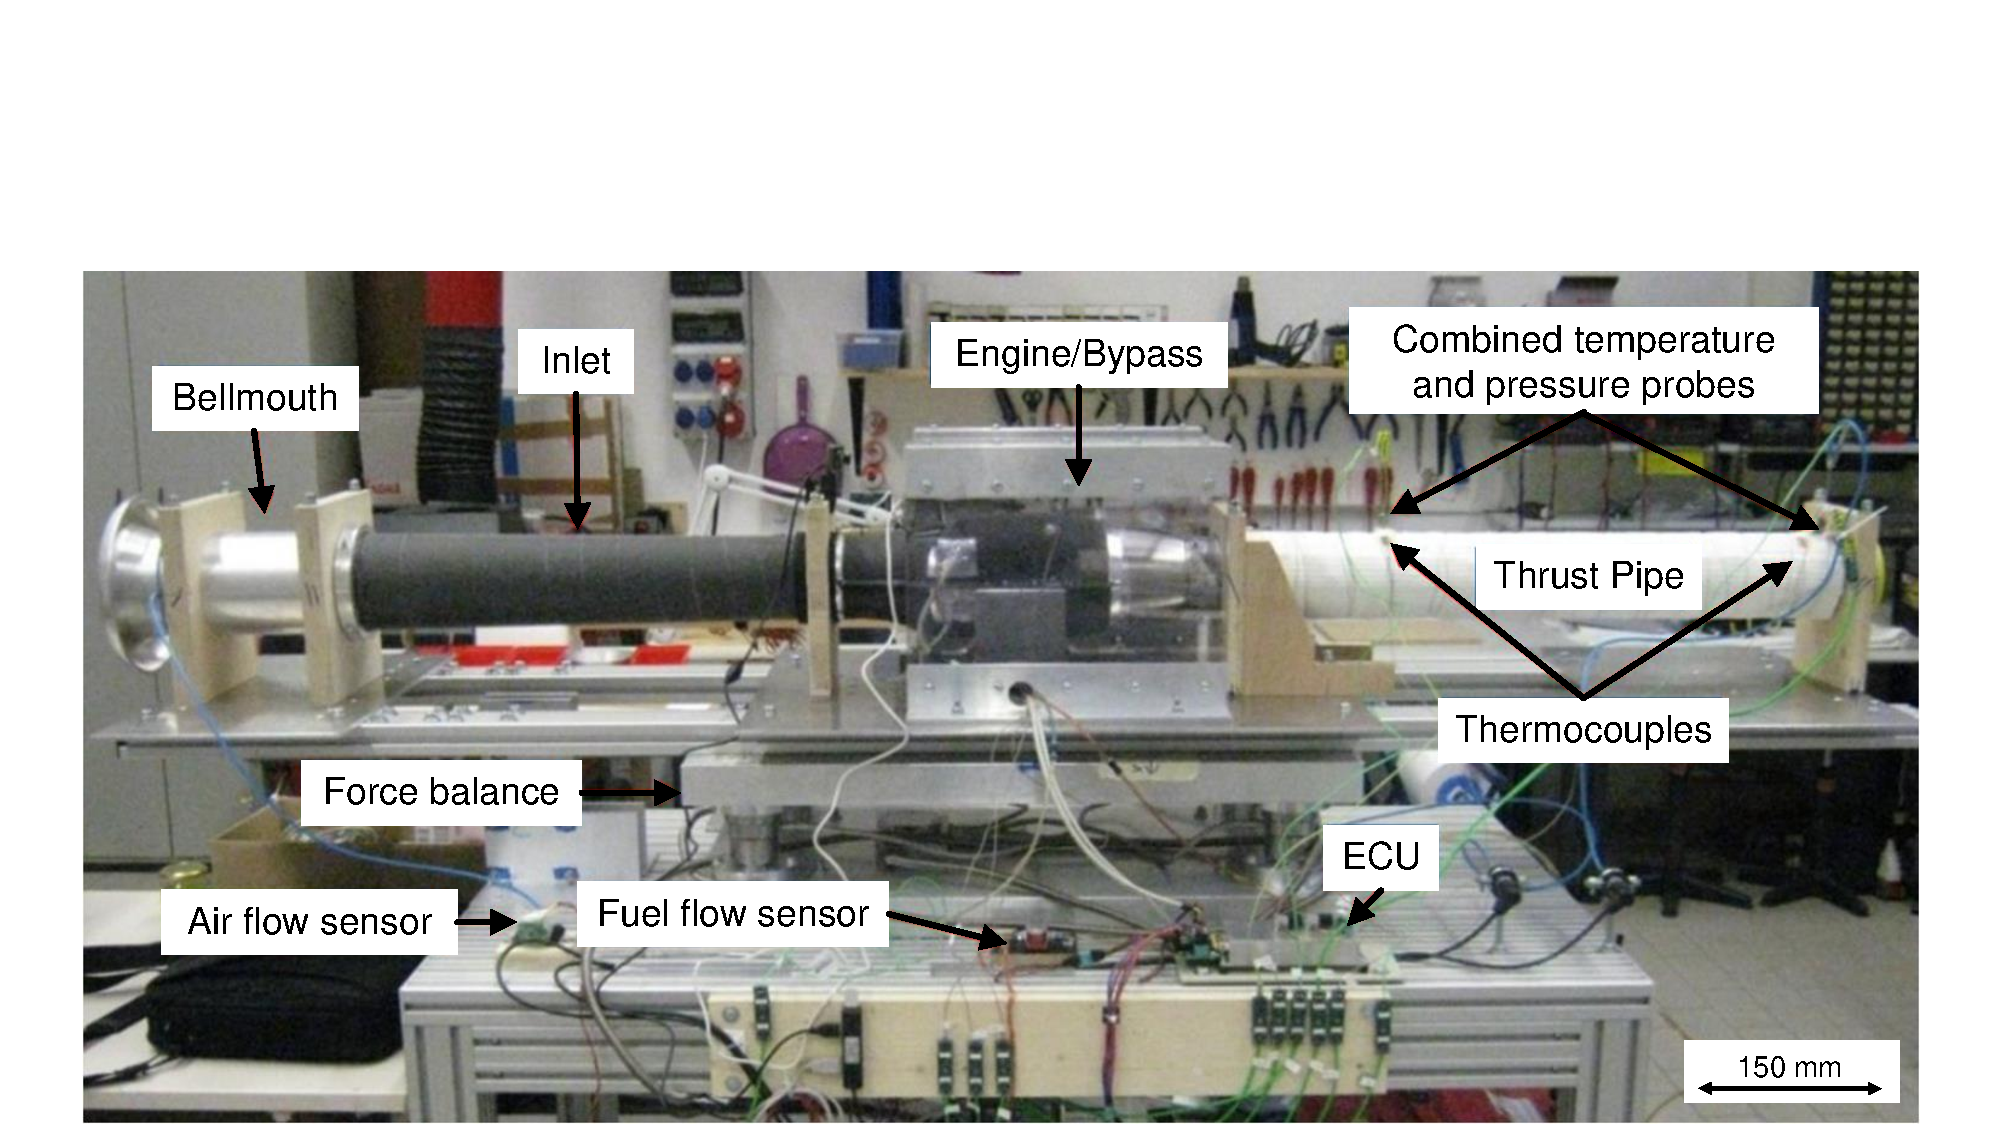
\includegraphics[trim = 15mm 0mm 15mm 45mm, clip,width=\textwidth]{Abbildungen/Triebwerkpruefstand}
	\caption{Foto vom Triebwerksprüfstand mit Maßstab und Beschriftung}
	\label{fig:Foto}
\end{figure}

\subsection{Diagramme}
Häufig werden Ergebnisse in wissenschaftlichen Ausarbeitungen mit Hilfe von Diagrammen (z.B. Liniendiagramme oder Balkendiagramme) dargestellt. Die Aussagekraft eines Diagramms hängt jedoch von verschiedenen Faktoren ab. Grundsätzlich gilt, dass in guten Diagrammen auf den ersten Blick die Kernaussage erkennbar ist und die Daten auch auf einem schwarz-weißen Ausdruck noch unterscheidbar sind. Schlechte Diagramme hingegen verwirren den Betrachter und/oder sind nur mit Hilfe einer Lupe interpretierbar.

Um ein Aussagekräftiges Diagramm zu erstellen, sollte zunächst anhand der Daten und der Kernaussage, die gemacht werden soll, ein Diagrammtyp ausgewählt werden: 
\begin{itemize}
\item Punkt-, Säulen- und Balkendiagramme sollten eingesetzt werden, wenn es zu den Daten keine Zwischenwerte gibt. 
\item Liniendiagramme hingegen sollten verwendet werden, wenn es Zwischenwerte zu den Daten gibt. 
\end{itemize}
Beim Vergleich von einer Simulation und einer Messung sollten die Ergebnisse der Simulation mit einem Liniendiagramm dargestellt werden (Simulationsergebnisse sind kontinuierlich) und die Messwerte mit einem Punktdiagramm (Messwerte sind diskret).

Ist der Diagrammtyp ausgewählt, sollten weiter folgende Hinweise beachtet werden:
\begin{itemize}
\item Die Schriftart sollte konsistent sein und zum Fließtext passen.
 \item Die Schriftgröße für Achsenbeschriftungen und die Legende darf nicht zu klein gewählt werden.
\item Achsen müssen immer mit Titel, Formelzeichen und Einheit (also z.B. Abstand x [m]) beschriftet werden.
\item Schraffuren sind zu vermeiden, besser sind verschiedene Grautöne. 
\item Diagramme mit zwei y-Achsen sollten vermieden werden. Falls in Ausnahmefällen doch zwei y-Achsen nötig sind, dann müssen die Kurven beschriftet werden, um eine klare Zuordnung zu den Achsen zu schaffen.
\item Die Darstellung von dreidimensionalen Strukturen, sollte vermieden werden. 3D-Diagramme sehen auf einem Bildschirm durchaus aussagekräftig aus, verlieren aber ihre Aussagekraft meist in einem Ausdruck.
\end{itemize}

\section{Einbindung von Formeln und Zahlen}
Formeln sind wie Abbildungen und Tabellen fortlaufend arabisch zu nummerieren. Die erste Ziffer der Nummerierung gibt das Kapitel an, die zweite Ziffer verweist auf die laufende Nummer innerhalb dieses Kapitels:
\begin{equation}
t_{gr} = \int_0^{V_{rot}} \frac{W_{to}}{g~(T-D_{to}-\mu(W_{to}-L_{to}))} dV\label{eq:xgroundroll}
\end{equation}
Formeln, die direkt übereinander stehen, sollen aneinander ausgerichtet werden.
\begin{align}
\frac{2 A_i}{GJ} = \frac{\oint_{i} \frac{q_i}{G_i t_i} ds}{T}-&\sum\limits_{j} \frac{\int_{(ij)} \frac{q_j}{G_ {ij} t_{ij}} ds}{T} ~~for ~i = 1,...,5 \label{eq:Torsion1}\\
&\sum\limits_{i=1}^5 2 A_i q_i = T \label{eq:Torsion2}
\end{align}
Bei Zahlen mit Einheiten gilt, dass zwischen Zahl und Einheit stets ein Leerzeichen steht, also z.B.: $19~\si{\percent}$, $8~\si{\metre}$, $5000~\si{\kilo\gram}$.

\section{Einbindung von Programm-Code}
Generell sollte die Verwendung von Programm-Code in der schriftlichen Ausarbeitung vermieden werden. Besser ist eine Darstellung von Algorithmen mit Formeln und Pseudocode sowie eine ausführlichen Beschreibung der Funktionsweise. Dies ermöglicht eine Erklärung der verwendeten Algorithmen, die unabhängig von der verwendeten Programmiersprache ist und sich leichter nachvollziehen lässt.

Dies kann Beispielsweise wie in Algorithmus \ref{alg:testalg} aussehen.
\begin{algorithm}[H]
	\caption{Ein Beispiel-Algorithmus}
	\label{alg:testalg}
	\begin{algorithmic}[1]
		\While{$\Delta\zeta > \text{Toleranz}$}
		\State calculate $\phi_{tip} = \sin \alpha$ \label{alglin:testline}
		\While{$\Delta\epsilon > \text{Toleranz}$} \Comment{minimize $\epsilon$}
		\State calculate something
		\EndWhile \Comment{$\epsilon$ is minimized}
		\State calculate $\alpha$
		\EndWhile \Comment{calculation finished}
	\end{algorithmic}
\end{algorithm}
Zeilen (z.B. Zeile \ref{alglin:testline}) können mit einem Label versehen und anschließend bei der Erläuterung referenziert werden. Kommentare können ebenfalls eingefügt werden. 

Lässt sich in Ausnahmefällen eine Verwendung von Quellcode aus \textsc{Matlab} oder anderen Programmen nicht vermeiden, sollte dieser mit Zeilennummern angegeben und anschließend erklärt werden:
\begin{spacing}{1.2}
\begin{lstlisting}[style=mlab,firstnumber = 1]{Name}
function Kosten = Example(in)
% Kostenfunktion
Kosten = sum((r_sim - r_flug).^2) + sum((diff(r_flug)-...
	diff(r_sim)).^2);
% Ausgabe
fprintf('%20.3f Kosten\n',Kosten);
end
\end{lstlisting}
\end{spacing}

%\section{Sonstige Hinweise zur Verwendung von Latex}
%Querverweise: in Kapitel~\ref{chap:wissA}
%
%Nummerierte Listen:
%\begin{enumerate}[noitemsep]
%\item ABC
%\item DEF
%\item GHI
%\end{enumerate}
%
%Auflistungen: 
%\begin{itemize}
%\item item a
%\item item b
%\item item c
%\end{itemize}
%
%Textformatierungen: \textbf{fett} \textit{kursiv} \underline{unterstrichen} 

\chapter{Abgabeprozedere}
Spätestens 6 Monate nach der Anmeldung der Arbeit muss diese elektronisch beim Betreuer zur Erstkorrektur abgegeben werden. Nach der Korrektur wird die Arbeit mit Anmerkungen zurückgegeben und kann nachgebessert werden. Anschließend ist die Studienarbeit ausgedruckt und gebunden beim Betreuer einzureichen. Auf der letzten Seite ist eine Daten-CD bzw. DVD mit allen relevanten Daten anzufügen. Diese beinhaltet u.A. folgende Elemente:
	\begin{itemize}
		\item Word-Datei bzw. kompilierbare Latex-Dateien der schriftlichen Ausarbeitung.
		\item PDF-Datei der schriftlichen Ausarbeitung.
		\item Verwendete Literatur und Literaturverwaltungsdateien (z.B. Citavi-Projekt).
		\item Alle in Zusammenhang mit der Arbeit erstellten Dokumente/Programme.
		\item Soweit bereits gehalten: Folien des Abschlussvortrags. 
		\item ...
	\end{itemize}
Zusätzlich zur Daten-CD bzw. DVD müssen alle Daten und Dokumente dem Betreuer elektronisch (via USB-Stick oder Sync \& Share) zur Verfügung gestellt werden.

\chapter{Abschlussvortrag}
Im Rahmen einer Bachelor-/Masterarbeit ist laut Prüfungsordnung ein Vortrag über das gestellte Thema zu halten. Für die Bearbeitung einer Semesterarbeit gilt dies nicht. In diesem Fall stellt es der LLS jedem Studenten frei, einen Vortrag über den Inhalt der Arbeit zu halten. Als Vorbereitung auf die Masterarbeit empfehlen wir jedoch diese Möglichkeit wahrzunehmen.

Der Ablauf am Vortragstag sieht folgendermaßen aus: Die Dauer des Vortrags beträgt 20 Minuten (+/- $10~\si{\percent}$). Nach Ablauf dieser Zeit wird der Vortrag vom Betreuer beendet. Im Anschluss an den Vortrag können Fragen gestellt werden und der Vortragende bekommt Feedback vom Betreuer.

Eine PowerPoint-Vorlage für die Präsentationsfolien wird vom Betreuer ausgegeben. Zur Erstellung der Folien wird weiterhin Folgendes empfohlen:
\begin{itemize}

\item Jede Folie ist in der Fußzeile mit einer Seitenzahl, Datum, Vorname und Nachname des Autors und dem Titel der Arbeit zu versehen.
\item Der Vortrag sollte ähnlich der schriftlichen Ausarbeitung eine Einleitung (Motivation, Vorgehensweise), einen theoretischen bzw. methodischen Teil, die praktische Umsetzung und eine abschließende Bewertung inklusive Zusammenfassung/Ausblick haben. 
\item Anzahl der Folien: Als Anhaltswert können je nach Vortragendem 1,5-2,5 Minuten pro Folie angesetzt werden. Dies hängt stark vom Inhalt der Folien und der Sprechgeschwindigkeit des Vortragenden ab. Es können sich somit maximal 15 Inhaltsfolien ergeben! 
\item Es ist darauf zu achten, dass zu jedem Zeitpunkt der Präsentation ein „roter Faden“ ersichtlich ist (zentrale Botschaft) und, dass jede Folie eine klare Aussage hat. 
 \item Gute Folien haben nicht mehr als drei Aufzählungspunkte je Überschrift und eine klare Gliederung, die auf den ersten Blick erkennbar ist. 
\item Achten Sie bei Abbildungen und Diagrammen auf gute Lesbarkeit der Daten und Achsenbeschriftungen. 
\end{itemize}
Ziehen Sie angemessene Kleidung an in der Sie sich wohlfühlen.


\pagebreak

\addcontentsline{toc}{chapter}{Literaturverzeichnis} % Bibliograhie wird im Inhaltsverzeichnis aufgeführt
\bibliography{Bibliographie} % Bibliographie wird aus der Datei Bibliographie eingeladen und erstellt
\bibliographystyle{agsm} % Zitierstil nach der Harvard-Methode

\chapter*{Eigenständigkeitserklärung} 
\markboth{Eigenständigkeitserklärung}{}
Hiermit versichere ich, dass ich die vorliegende Arbeit selbstständig und ausschließlich unter Zuhilfenahme der im Literaturverzeichnis angegebenen Quellen angefertigt habe. Aus anderen Publikationen und Veröffentlichungen entnommenen Ideen, Abbildungen und Textstellen sind als solche direkt kenntlich gemacht. Die Arbeit ist in gleicher oder ähnlicher Form noch keiner Prüfungsbehörde vorgelegt worden. 

\begin{figure}[h]
\begin{minipage}[t]{0.45\textwidth}
\vspace{0.1\textheight}
  Garching, den xx. Januar 20xx
\end{minipage}
%\hfilll
\begin{minipage}[t]{0.45\textwidth}
\begin{flushright}
  \vspace{0.13\textheight}
  \hrulefill
  \begin{center}
  Vorname Nachname
  \end{center}
\end{flushright}
\end{minipage}
\end{figure}

%%%%%%%%%%%%%%%%%%%%%%%%%%%%%%%%Anhang%%%%%%%%%%%%%%%%%%%%%%%%%%%%%%%%%%%%%%%
\renewcommand{\thechapter}{\Alph} % Kapitel Nummerierung mit Buchstaben
\appendix

\chapter{Anhang: Information über den E-Fan}
\markboth{A Anhang: Information über den E-Fan}{} %Was in the Kopfzeile angezeigt wird

\pagenumbering{arabic} % Arabische Seitennummerierung
\setcounter{page}{1}
\renewcommand{\thepage}{\thechapter-\arabic{page}} % Seitennummerierung mit A-1, A-2, etc.
\renewcommand\thefigure{\Alph{chapter}.\arabic{figure}} 
 \setcounter{figure}{0} 
\renewcommand\thetable{\Alph{chapter}.\arabic{table}} 
 \setcounter{table}{0} 

Der Anhang enthält Informationen zur Arbeit, die aber zu umfangreich sind, um in die eigentlichen Kapitel aufgenommen zu werden (z.B. Versuchsprotokolle, technische Zeichnungen, Produktdatenblätter etc). Er wird als letztes Kapitel aufgeführt und in gleicher Weise (ggf. mit Unterkapiteln) durchnummeriert wie der Hauptteil der Arbeit. Im Inhaltsverzeichnis werden Unterkapitel des Anhangs im Gegensatz zum Hauptteil nicht aufgeführt.

\stoptocwriting % do not include sections in Table of Content

\section{3-Ansichten Zeichnung des E-Fan 1.0}
\begin{figure}[H]
	\centering
	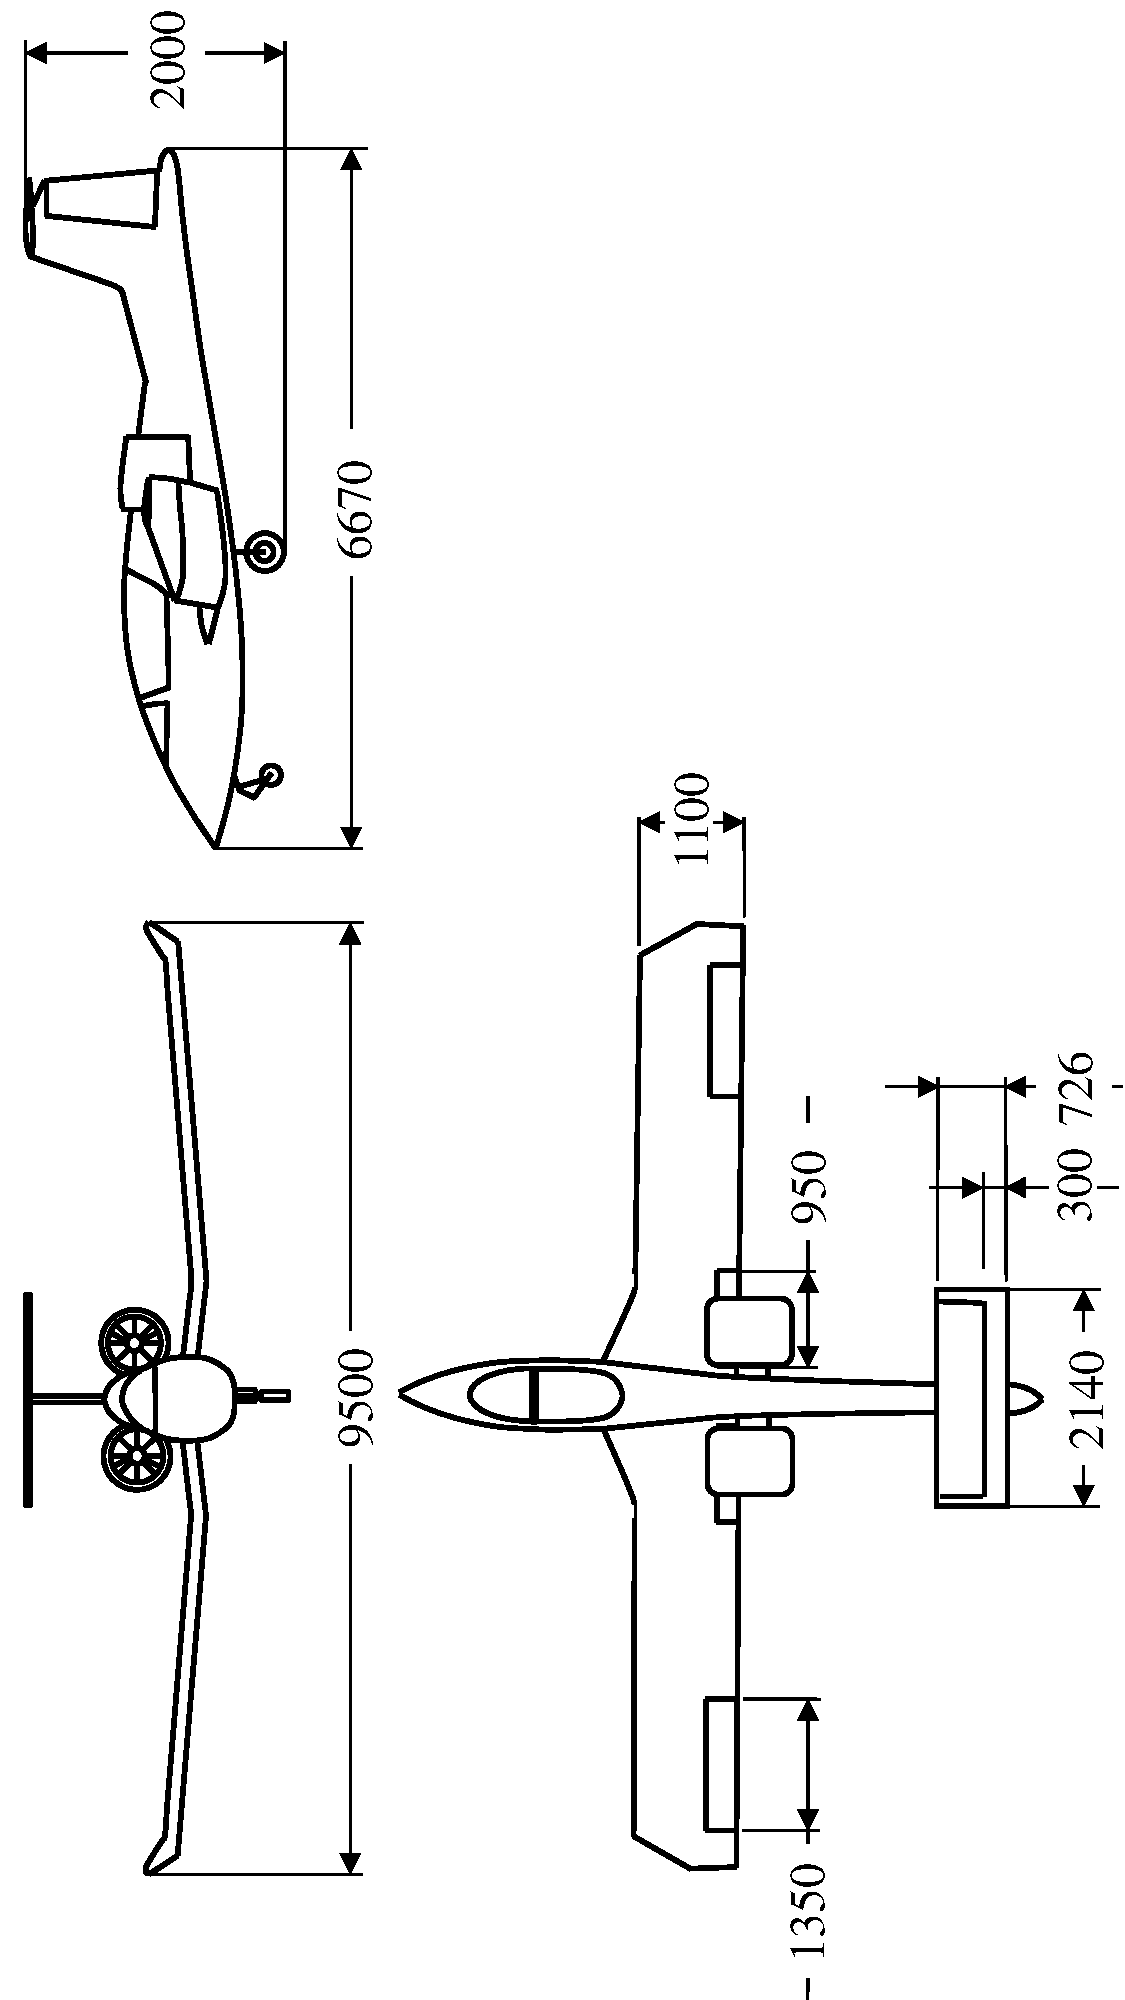
\includegraphics[trim = 0mm 0mm 0mm 0mm, clip,width=0.5\textwidth]{Anhang/3views_EFan}
	\caption[]{3-Ansichten Zeichnung des E-Fan 1.0 (alle Maße in [$\si{\milli\metre}$])}
	\label{fig:3views}
\end{figure}

\section{Versuchsprotokoll}
Protokoll

\resumetocwriting % include sections in Table of Content
\end{document}
